\newpage
\section[Фигура 2]{Фигура 2}

Строим круг и зведу, используя примитивы \textbf{Inkscape}. 
Применяем выравнивание.
Применяем операцию \textit{\textbf{Intersection (пересечение)}}. 
Производим заливку фигуры, инструмент \textit{\textbf{Fill and Stroke}}.
\begin{figure}[H]
    \begin{minipage}[h]{0.47\linewidth}
        \center{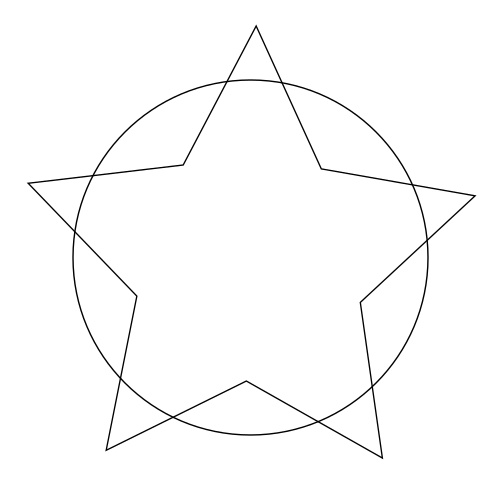
\includegraphics[width=1\linewidth]{2_1_create.png}} Создание фигур\\
    \end{minipage}
    \hfill
    \begin{minipage}[h]{0.47\linewidth}
        \center{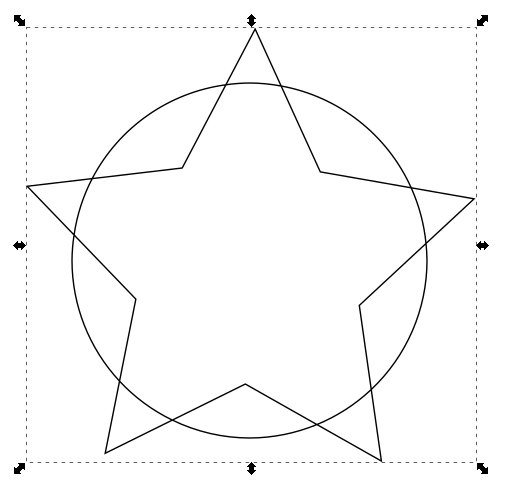
\includegraphics[width=1\linewidth]{2_2_intersection.png}}\\ Операция Intersection
    \end{minipage}
    \hfill
    \centering
    \begin{minipage}[h]{0.47\linewidth}
        \center{
\includegraphics[width=1\linewidth]{2_3_fill.png}} Использование Fill and Stroke
    \end{minipage}
\end{figure}
